\documentclass[a4paper]{article}
\usepackage{graphicx}
\usepackage{amsmath, amsfonts, geometry, float, listings, enumerate, multicol}
\usepackage{multicol, float, color, colortbl}
\usepackage{tikz, titlesec, parskip, pgfplots, filecontents}
\usepackage{hyperref}
\usepackage{amsmath}
\usepackage{tikz, titlesec, parskip}
\usepackage{tikz,pgfplots}
\usepackage{stackengine}
\usepackage{amsmath}
\usepackage{tikz} 
\usepackage[americanvoltages,fulldiodes,siunitx]{circuitikz}
\usetikzlibrary{shapes,arrows}
\usepackage{enumitem}
\usepackage{amssymb}
\titlespacing{\section}{0pt}{10pt}{0pt}
\titlespacing{\subsection}{0pt}{10pt}{0pt}
\titlespacing{\subsubsection}{0pt}{10pt}{0pt}

\usetikzlibrary{calc,patterns,through}
\newcommand{\arcangle}{%
	\mathord{<\mspace{-9mu}\mathrel{)}\mspace{2mu}}%
}
\newcommand{\LRT}[2]{%
	\mathrel{\mathop\gtrless\limits^{#1}_{#2}}%
}
\renewcommand{\baselinestretch}{1.4}
 \geometry{
 a4paper,
 total={170mm,257mm},
 left=20mm,
 top=20mm,
 }
\usepackage{fancyhdr}
\usepackage{indentfirst}
\pagestyle{fancy}
\fancyhf{}
\rhead{\textbf{آمار و احتمال مهندسی}}
\lhead{\textbf{تمرین عملی سری دوم}}
\cfoot{(\space \space \space \space \textbf{\thepage}  \space \space \space)}
\renewcommand{\headrulewidth}{1pt}
\renewcommand{\footrulewidth}{1pt}

 
\usepackage{xepersian}
\setlatintextfont{Times New Roman}
\settextfont{XB Niloofar}
\setdigitfont{XB Niloofar}
\DefaultMathsDigits

\makeatletter
\bidi@patchcmd{\@Abjad}{آ}{الف}
{\typeout{Succeeded in changing آ into الف}}
{\typeout{Failed in changing آ into الف}}
\makeatother
\PersianAlphs

\begin{document}
\begin{minipage}{0.6\textwidth}
\begin{bf}
\begin{center}
	به نام خدا\\
	\vspace{0.25cm}
	دانشگاه صنعتی شریف\\
	\vspace{0.25cm}
	دانشکده مهندسی برق\\
	\vspace{0.5cm}

\large
گروه دکتر یاسایی - آمار و احتمال مهندسی \\
نیم سال اول
۱۴۰۱-۱۴۰۰\\
\Large
\vspace{0.4cm}
تمرین عملی سری دوم\\
\end{center}
\end{bf}
\normalsize
\end{minipage} \hfill
\begin{minipage}{0.35\textwidth}
\begin{flushleft}
\includegraphics[width=0.6\textwidth]{Shariflogo.png}\\ \large
\end{flushleft}

 \end{minipage}
\\

\rule[0.1\baselineskip]{\textwidth}{1.5pt}

\large

\section*{
لطفاً به نکات زیر توجه بفرمایید:
}
\begin{enumerate}
	\item 
نتایج و پاسخ های خود را در یک فایل با فرمت zip به نام
\LR{HW$2$-Name-StudentNumber}
 در سایت  cw قرار دهید.
	\item 
کسب نمره کامل در هر سؤال مستلزم تحویل  \textbf{کدها} و \textbf{توضیحات} می‌باشد. 
\item 
برای سؤالات، باید روشی که استفاده کرده‌اید را توضیح  و نتایجی که گرفته‌اید را ارائه دهید. این توضیحات می‌تواند در یک فایل  pdf  و یا در یک فایل  ipynb باشد. 
\item 
کدهای خود را خوانا بنویسید و کامنت‌‌گذاری کنید. در plot های خود عنوان، label و خط‌کشی‌های مناسب را اضافه کنید.
\item
ابهام يا اشكالات خود را مي توانيد  از طریق
\href{https://t.me/Amirhosein_javadi}{@Amirhosein\_Javadi}
یا 
\href{mailto:javadiamirhosein.2000@gmail.com}{\LR{Javadiamirhosein.$2000$@gmail.com}}
مطرح نماييد.
\item 
کدهای شما تماماً باید توسط خودتان نوشته شده باشند. هرگونه استفاده از کد دیگران به هر شکل ممکن، تقلب محسوب می‌شود و نمره تمرین کامپیوتری جاری صفر خواهد شد. پس در هیچ صورت کدهای خود را برای دیگران ارسال نکنید.

\item 
مهلت تحویل:  
\end{enumerate}
\clearpage
\section{
حرکت براونی و توزیع نرمال
}
در این سوال قصد داریم با توزیع نرمال و حرکت براونی بیشتر آشنا شویم.
فرض کنید ذره‌ای در هر واحد زمانی
$ \delta $ 
ثانیه‌ای به اندازه‌ی 
$ \epsilon $
با احتمال برابر به سمت راست یا چپ حرکت می‌کند و هدف ما پیدا کردن مکان ذره در زمان $ t $،
$ B_{t} $، 
است. 
\begin{enumerate}
	\item
زمان را با نرخ $ 10000 $ سمپل بر ثانیه نمونه برداری کنید. فاصله‌ی بین هر دو نمونه در واقع همان $ \delta $ مسئله است و در کدام از این بازه‌های زمانی‌ به اندازه‌ی 
$ \epsilon = \frac{2}{100} $ 
حرکت کنید. 
	\item
حال میتوانید تابعی تعریف کنید که خروجی آن متغیر تصادفی از مکان ذره در زمان 
$ t = 1 $
باشد. 
این تابع را 
$ 10000 $
بار اجرا کنید و در یک نمودار هیستوگرامی از 
$ B_{1} $
رسم کنید. انتظار دارید این هیستوگرام متناظر با چگالی احتمال چه متغیر تصادفی با چه پارامترهایی باشد؟ تابع چگالی احتمال این متغیر تصادفی را هم در همین نمودار رسم کنید.
	\item
	قسمت دوم را برای 
$ B_{2} $،	
$ B_{3} $،
$ B_{4} $
تکرار کنید.
	
\end{enumerate}	
\section{ 
تخمین پارامتر $ p $ متغیر تصادفی برنولی
}
در این سوال قصد داریم با کمک تخمینگر 
\lr{Maximum Likelihood}
پارامتر $ p $ یک متغیر تصادفی برنولی را حدس بزنیم.
\begin{enumerate}
	\item 
تابعی بنویسید که در هر اجرای آن، عدد تصادفی $ p $ بین $ 0 $ تا $ 1 $ به صورت تصادفی یکنواخت انتخاب کند. سپس 
$ n = 1000 $ 
نمونه از متغیر تصادفی برنولی با پارامتر $ p  $ بردارید و در آرایه‌ای با نام Samples ذخیره کنید. آرایه‌ای به نام 
\lr{ML\_Estimator}
به طول $ n $ تعریف کنید و درایه‌ی $ i $ام آن را برابر خروجی تخمینگر  
\lr{Maximum Likelihood}
در حالتی که فقط $ i $ درایه‌ی اول آرایه‌ی Samples را میدانید، قرار دهید. آرایه‌ی خطای تخیمنگر را برابر قدر مطلق اختلاف هر درایه‌ی 
\lr{ML\_Estimator}
و 
 p  
 قرار دهید و این آرایه را به عنوان خروجی تابع تعیین کنید. در یک نمودار خطای تخمینگر را رسم کنید.
	 \item 
تابع بالا را $ 1000 $ بار تکرار کنید و خطای میانگین در این $ 1000 $ تکرار را به دست بیاورید. در یک نمودار خطای میانگین تخمینگر را رسم کنید.
\end{enumerate}

\section{ 
تخمین پارامترهای  $ \mu $ و $ \sigma $ متغیر تصادفی نرمال
}
در این سوال قصد داریم با کمک تخمینگر 
\lr{Maximum Likelihood}
پارامترها  $ \mu $ و $ \sigma $
یک متغیر تصادفی نرمال را حدس بزنیم. تابعی بنویسید که در هر اجرای آن، عدد تصادفی 
$ \mu $ 
و 
$ \sigma $
را به صورت تصادفی یکنواخت از بازه‌ی 
$ [-2,2] $
و
$ [0,5] $
 انتخاب کند و این دو عدد را چاپ کند. سپس 
 $ n = 1000 $ 
 نمونه از متغیر تصادفی نمایی
 $ \mathbb{N}(\mu,\sigma^{2}) $
 بردارید و در آرایه‌ای با نام Samples ذخیره کنید.
  آرایه‌ای به نام 
 \lr{Mu\_Estimator}
 و
 \lr{Sigma\_Estimator}
 به طول $ n $ تعریف کنید و درایه‌ی $ i $ام آن را برابر خروجی تخمینگر  
 \lr{Maximum Likelihood}
 در حالتی که فقط $ i $ درایه‌ی اول آرایه‌ی Samples را میدانید، قرار دهید. دقت کنید که از 
 $ \mu $ 
 و 
 $ \sigma $
 نمیتوانید برای این تخمین استفاده کنید. 
 آرایه‌ی خطای تخیمنگر $ \mu $ را برابر قدر مطلق اختلاف هر درایه‌ی 
 \lr{Mu\_Estimator}
 و 
$ \mu $
 و آرایه‌ی خطای تخیمنگر $ \sigma $ را برابر قدر مطلق اختلاف هر درایه‌ی 
\lr{Sigma\_Estimator}
 و 
$ \sigma $
 قرار دهید.
 بهترین تخمین از 
  $ \mu $ 
 و 
 $ \sigma $
 را چاپ کنید. 
این دو آرایه را به عنوان خروجی‌های تابع تعیین کنید. در دو نمودار این دو خطای تخمینگر را رسم کنید.
\newpage
\section{تست فرضیه}
در این سوال قصد داریم با مفهوم 
\lr{hypothesis testing}
بیشتر آشنا شویم. فرض کنید دو متغیر تصادفی نرمال
 $ H_{0} $ 
 و
 $ {H}_{1} $ 
 به صورت زیر داریم. 
\begin{equation}
 	H_{0} \sim \mathbb{N} (\mu = -1, \sigma = 5)
\end{equation}
\begin{equation}
 	{H}_{1} \sim \mathbb{N} (\mu = 1, \sigma = 5)
\end{equation}
\begin{enumerate}
	\item 
	تابع چگالی احتمال 
	 $ {H}_{0} $ 
	و
	$ {H}_{1} $ 
	را در یک نمودار رسم کنید. 
	\item 
	همان‌ طور که در درس دیدیم برای حدس زدن مدل بین 
	 $ {H}_{0} $ 
و
	$ {H}_{1} $ 
	با داشتن نمونه‌ی 
$ x $	
	میتوانیم از تست زیر استفاده کنیم:
	\begin{equation}
		f_{{H}_{1}} \LRT{H_1}{H_0} f_{{H}_{0}} \Leftrightarrow (x+1)^{2} \LRT{H_1}{H_0} (x-1)^{2} \Leftrightarrow 2x \LRT{H_1}{H_0} -2x
	\label{test1}	
	\end{equation} 
در این سوال قصد داریم بررسی کنیم آیا با نمونه‌‌های بیشتر میتوانیم مدل‌های 
$ {H}_{0} $ 
و
$ {H}_{1} $ 
را بهتر از هم جدا کنیم یا نه. به همین منظور با داشته داده‌های 
$ x_{i=1:n} $
تست 
\ref{test1}
را به تست زیر تعمیم می‌دهیم.
	\begin{equation}
	f_{{H}_{1}} \LRT{H_1}{H_0} f_{{H}_{0}} \Leftrightarrow \sum_{i=1}^{n}(x_{i}+1)^{2} \LRT{H_1}{H_0} \sum_{i=1}^{n}(x_{i}-1)^{2} \Leftrightarrow \sum_{i=1}^{n} 2 x_{i}  \LRT{H_1}{H_0} \sum_{i=1}^{n} -2 x_{i} 
	\label{test2}	
	\end{equation}

برای این کار تابعی بنویسید که یک آرایه به نام 
\lr{Indicator}
شامل
 $ n = 100 $
  نمونه از متغیر تصادفی برنولی با پارامتر 
$ \dfrac{1}{2} $
تولید کند. حال $ n $ آزمایش انجام می‌دهیم و در هر آزمایش سعی داریم 
درایه‌ی $ i $ام آرایه‌ی 
\lr{Indicator}
را حدس بزنیم. همچنین داریم:
\begin{equation}
	H^{i} = \begin{cases}
		H_{1} & Indicator[i] = 1
		\\
		H_{0} & Indicator[i] = 0
	\end{cases}
\end{equation}
پس در هر آزمایش 
$ H^{i} $
را تعیین کنید و برای هر 
$ H^{i} $
تست زیر را $ 10000 $ بار تکرار کنید.
\\
 از مدل مربوطه $ i $ نمونه‌ ‌بگیرید. حال تست 
\ref{test2}
را اجرا کنید و تخمین خود را از درایه‌ی $ i $ام آرایه‌ی  
\lr{Indicator}
به دست بیاورید و در یک آرایه به نام 
\lr{Estimation}
ذخیره کنید. 
خطای تخمین برابر قدرمطلق اختلاف بین 
\lr{Indicator}
و
\lr{Estimation}
است. 

 در یک نمودار میانگین خطا در $ 10000 $ تست را به ازای $ i $ نمونه رسم کنید. 	
\end{enumerate}

\section{ جمع رئوس}
گراف زیر را در نظر بگیرید. هر کدام از رئوس این گراف یک عدد مخصوص دارد و هدف ما پیدا کردن مجموع عددهای رئوس این گراف  در هر راس از گراف است. در اینجا هر راس می‌تواند با راس همسایه تبادل اطلاعات کند ولی رئوس حافظه محدودی دارند و می‌توانند فقط تعداد محدودی عدد در خود ذخیره کنند. یال‌ها به دلخواه شماره‌گذاری شده‌اند و عدد هر راس داخل آن در پرانتز نوشته شده‌است. 
\begin{center}
		
	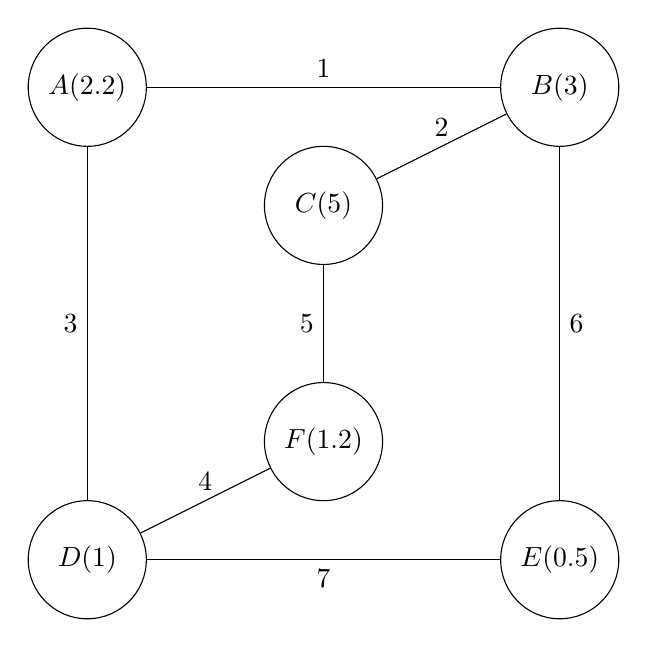
\begin{tikzpicture}[main/.style = {draw, circle, minimum width=15mm, minimum height=15mm}] 
		\node (1) [main]  at (1.5,6) {$A(2.2)$};
		\node (2) [main]  at (7.5,6) {$B(3)$};
		\node (3) [main]  at (4.5,4.5) {$C(5)$};
		\node (4) [main]  at (1.5,0) {$D(1)$};
		\node (5) [main]  at (7.5,0) {$E(0.5)$};
		\node (6) [main]  at (4.5,1.5) {$F(1.2)$};
		\draw[-]  (1) -- (2) node[midway,above] {$1$};
		\draw[-]  (2) -- (3) node[midway,above] {$2$};
		\draw[-]  (1) -- (4) node[midway,left] {$3$};
		\draw[-]  (6) -- (4) node[midway,above] {$4$};
		\draw[-]  (3) -- (6) node[midway,left] {$5$};
		\draw[-]  (2) -- (5) node[midway,right] {$6$};
		\draw[-]  (4) -- (5) node[midway,below] {$7$};
	\end{tikzpicture} 
\end{center}
یک ایده‌ برای تخمین مجموع مقادیر رئوس این است که هر راس نمونه‌ی تصادفی از متغیر تصادفی نمایی با  با نرخ عدد آن راس  تولید کند و نمونه‌ی خود را با راس همسایه تبادل ‌کند و پس از آن دو راس همسایه نمونه‌ی خود را با مینیمم نمونه‌ی خود و همسایه جایگزین ‌کنند. پس از چند مرحله همه رئوس مینیمم نمونه‌های تصادفی گره‌های مختلف را میبینند و الگوریتم همگرا می‌شوند و گره‌ها میتوانند مقدار مینیمم را ذخیره ‌کنند. حال می‌دانیم مینیمم $ n $ متغیر تصادفی نمایی با نرخ‌های 
$ \lambda_{i} $،
 یک متغیر تصادفی نمایی با نرخ 
$ \sum_{i=1}^{n} \lambda_{i} $ 
است. پس اگر تعداد مناسبی این الگوریتم را تکرار کنیم، همه رئوس به چند نمونه iid از متغیر نمایی با پارامتر مجموع مطلوب ما دسترسی دارند و می‌توانند با تخمین 
\lr{Maximum Likelihood}
 پارامتر نرخ متغیر نمایی را تخمین بزنند.
\begin{enumerate}
	\item 
می‌توانید یال‌ها را شماره‌گذاری کنید یا از شماره‌گذاری پیشنهادی استفاده کنید. در هر راند به ترتیب‌، یالی را انتخاب کنید و بین دو نمونه‌ی رئوس دو سر یال مینیمم‌گیری کنید و در صورت نیاز نمونه‌ی رئوس را به روز رسانی کنید. 
	\item 
حداقل تعداد راند مورد نیاز برای این که مطمئن شویم نمونه‌ی مینیمم به همه‌ی گره‌ها رسیده است چه قدر است؟ 
	\item 
الگوریتم بالا را اجرا کنید و مجموع اعداد رئوس را با حداکثر خطای $ 0.1 $ به دست بیاورید.
\end{enumerate}
\end{document}
